\documentclass[conference]{IEEEtran}
\IEEEoverridecommandlockouts
\usepackage[T1]{fontenc}
\usepackage{newtxtext,newtxmath}

\usepackage{amsmath}
\usepackage{graphicx}
\usepackage{textcomp}
\usepackage{xcolor}
\usepackage{booktabs}
\usepackage{array}
\usepackage{algorithm}
\usepackage{algpseudocode}
\usepackage{tikz}
\usetikzlibrary{positioning,arrows.meta,fit,shapes.misc}
\usepackage[hidelinks]{hyperref}
\usepackage{url}
\def\UrlFont{\ttfamily\small}

% =====================================================================
%  EDIT HERE: names, roles (shown under each name) and affiliation.
%  Change only the text inside the braces; nothing else needs to move.
% =====================================================================
\newcommand{\AuthorOneName}{Pranay Vishwakarma}
\newcommand{\AuthorOneRole}{Team Leader}
\newcommand{\AuthorTwoName}{Vaiditya Tanwar}
\newcommand{\AuthorTwoRole}{Architecture \& CI Lead}
\newcommand{\AuthorThreeName}{Vishesh Rao}
\newcommand{\AuthorThreeRole}{Package \& Release Setup}
\newcommand{\AuthorFourName}{Sayan Bhattacharya}
\newcommand{\AuthorFourRole}{Documentation \& Report}

\newcommand{\Department}{Department of Computer Science and Artificial Intelligence (CSAI)}
\newcommand{\Institute}{Newton School of Technology, Rishihood University}
\newcommand{\Location}{Sonipat, India}
\newcommand{\ReportLine}{Hacktoberfest 2026, Hack Day Sonipat --- Team Cappybara Project Report}

% Short roles used in the Individual Contributions table (Appendix B)
\newcommand{\AuthorOneWork}{Project leadership; website shell foundation (\texttt{src/viewer/shell.mjs}) and its tests}
\newcommand{\AuthorTwoWork}{Architecture and contract documentation; CI workflow; gated release, readiness and candidate tooling}
\newcommand{\AuthorThreeWork}{Scoped npm package identity and metadata (\texttt{@xagents\_in/unmask})}
\newcommand{\AuthorFourWork}{Repository analysis and this IEEE-format project report}
% =====================================================================

\newcommand{\code}[1]{\texttt{#1}}
\makeatletter
\newcommand{\linebreakand}{%
  \end{@IEEEauthorhalign}\hfill\mbox{}\par\mbox{}\hfill\begin{@IEEEauthorhalign}}
\makeatother

\begin{document}

\title{UNMASK: Evidence-Bounded Comparison of\\
Published npm Packages Against Their Source\\
Repositories for Supply-Chain Review}

\author{%
\IEEEauthorblockN{\AuthorOneName}
\IEEEauthorblockA{\AuthorOneRole}
\and
\IEEEauthorblockN{\AuthorTwoName}
\IEEEauthorblockA{\AuthorTwoRole}
\and
\IEEEauthorblockN{\AuthorThreeName}
\IEEEauthorblockA{\AuthorThreeRole}
\and
\IEEEauthorblockN{\AuthorFourName}
\IEEEauthorblockA{\AuthorFourRole}
\linebreakand
\IEEEauthorblockA{\textit{\Department}\\
\textit{\Institute}, \Location\\
\ReportLine}
}

\maketitle

\begin{abstract}
A published software package is a separate artifact from the repository that
claims to produce it. Nothing in the npm registry forces the two to agree, and
several high-profile attacks have shipped code in the tarball that never appeared
in reviewed source. This report describes UNMASK, a package-integrity analyzer
built by Team Cappybara for Problem~04 of Hacktoberfest 2026 (Hack Day
Sonipat): \emph{Published Package vs Source Code Integrity Analyzer}. UNMASK
inventories an npm tarball and a source archive pinned to a full commit SHA
without executing either, classifies every regular file of the artifact into one
of four correspondence states (byte-identical, changed, artifact-only,
not-compared), binds each observation to a byte range in a digest-addressed
blob, and derives a deterministic exit code from a small, versioned policy. An
optional large language model (Google Gemma) may explain the evidence, but its
output is advisory, must quote supplied evidence verbatim, and can never clear a
deterministic finding. We present the threat model, the separated-facts design
principle, the archive and correspondence algorithms, the hosted process model
and the release pipeline that binds a source commit, an npm tarball and a
container image digest. We report the state of the repository honestly: the
merged main branch contains the engineering scaffold (CI, 43 test declarations
across nine files, a gated release pipeline and the website shell), while the
analyzer core is specified but pending merge, and hosted model generation is
blocked by an HTTP~403 quota error. We close with a measurable evaluation plan.
\end{abstract}

\begin{IEEEkeywords}
software supply chain, npm, package integrity, reproducible builds, provenance,
static analysis, large language models, evidence grounding, CI/CD
\end{IEEEkeywords}

\section{Introduction}

\IEEEPARstart{D}{evelopers} install packages, not repositories. When a team
reviews a dependency it usually reads the GitHub source, yet what actually runs
is the tarball downloaded from the registry. The two are linked only by
convention: the publisher runs \code{npm publish} on a machine the reviewer
never sees, possibly after a build, minification or a manual edit. Two
properties make this gap dangerous. First, it is invisible by default:
\code{npm install} verifies that the tarball matches the registry's recorded
hash, not that it matches any source. Second, it has been exploited repeatedly,
from the \code{event-stream} incident, where a malicious payload lived only in
the published build of a dependency~\cite{eventstream}, to the \code{xz-utils}
backdoor, whose trigger was present in release tarballs but not in the
corresponding Git tree~\cite{xz}.

Existing responses fall into two families. \emph{Attestation} approaches such
as Sigstore~\cite{sigstore}, in-toto~\cite{intoto}, SLSA~\cite{slsa} and npm
provenance~\cite{npmprov} sign statements about how an artifact was built; they
are strong when adopted but say nothing about the large majority of packages
that publish no attestation. \emph{Reproduction} approaches rebuild the artifact
from source and compare~\cite{lamb2021}; they are definitive when they succeed
but require executing untrusted build scripts and a faithful toolchain. A
reviewer facing an arbitrary package today needs a third option: an inert,
bounded, explainable comparison that states exactly what is known and what is
not.

This project addresses three design questions under a single, documented
contract:
\begin{description}
\item[\textbf{DQ1}] Can the difference between a published npm tarball and a
pinned source archive be computed \emph{without executing} either, under explicit
resource bounds, and still be useful to a reviewer?
\item[\textbf{DQ2}] How should the result separate facts of different strength
(registry integrity, source claim, byte correspondence, syntax cues, model
hypotheses) so that no weaker fact silently upgrades a stronger one?
\item[\textbf{DQ3}] Under what constraints can a hosted LLM add explanation
value without becoming a trusted classifier?
\end{description}

The contributions of this phase are: (i) a threat model and a
\emph{separated-facts} principle that governs every report field; (ii) a
specified, bounded archive inventory and a four-state correspondence
classification with byte-range evidence; (iii) a deterministic, versioned exit
policy that is independent of the model; (iv) an advisory model contract with
mandatory verbatim citations; (v) a CI and release pipeline that binds source
commit, npm tarball and image digest; and (vi) an honest status audit and a
measurable plan for evaluation.

The remainder of the report is organised as follows. Section~\ref{sec:lit}
reviews related work. Section~\ref{sec:problem} states the problem and threat
model, and Section~\ref{sec:design} the requirements and design decisions.
Section~\ref{sec:arch} describes the architecture, Section~\ref{sec:method} the
core methods, and Section~\ref{sec:eng} the engineering and evaluation design.
Section~\ref{sec:status} reports the current status, Section~\ref{sec:disc}
discusses the design and alternatives, and Section~\ref{sec:future} sets out
limitations and future work.

\section{Literature Review}\label{sec:lit}

\subsection{Attacks on Package Ecosystems}
Zimmermann et al.~\cite{zimmermann2019} showed that the npm dependency graph is
a ``small world'': a handful of maintainer accounts can reach a large fraction
of all packages, so a single compromised publisher has outsized reach. Ohm et
al.~\cite{ohm2020} catalogued 174 malicious packages and found that most
injected code runs at install time through lifecycle hooks or on first import.
Duan et al.~\cite{duan2021} built a measurement pipeline across npm, PyPI and
RubyGems and confirmed hundreds of previously unknown malicious packages. These
studies motivate two UNMASK choices: install hooks are first-class policy
findings, and no target code is ever executed.

\subsection{Source-to-Package Discrepancy}
The work closest to ours is LastPyMile~\cite{vu2021}, which compared PyPI
artifacts with their GitHub repositories and found that discrepancies are
common and mostly benign (generated files, packaging metadata), while malicious
injections hide among them. Vu et al.\ therefore argue that a useful tool must
\emph{explain} differences, not merely list them. UNMASK adopts this framing for
npm and adds explicit byte-level evidence and a model-independent policy.

\subsection{Provenance and Attestation}
in-toto~\cite{intoto} records signed layouts of supply-chain steps; Sigstore~\cite{sigstore}
removes long-lived signing keys through short-lived certificates and a
transparency log; SLSA~\cite{slsa} grades build integrity in levels. npm now
records Sigstore-backed provenance for packages published from supported CI
systems~\cite{npmprov}. UNMASK records such claims as \emph{labels} and states
explicitly when they were not cryptographically verified.

\subsection{Reproducible Builds}
Lamb and Zacchiroli~\cite{lamb2021} describe reproducible builds as the
strongest practical guarantee that a binary corresponds to its source. Their
cost is a faithful, deterministic toolchain and the execution of build scripts.
UNMASK deliberately stops short of rebuilding and makes no claim of build
equivalence; it measures byte correspondence only.

\subsection{LLMs for Security Explanation}
Large language models can summarise code and suggest hypotheses, but they
hallucinate, including invented code and citations~\cite{ji2023}. Retrieval and
citation grounding reduce, but do not remove, this risk~\cite{gao2023}. The
selected model family, Gemma~\cite{gemma}, is open-weight, which aids
inspectability. UNMASK therefore restricts the model to bounded evidence and
validates that every quotation exists at its claimed location.

\subsection{Research Gap}
Attestation covers packages that opt in; reproduction covers packages whose
builds can be replayed; discrepancy studies measure ecosystems in aggregate.
Few tools give an individual reviewer a bounded, non-executing, per-file
comparison whose every claim is tied to evidence and whose verdict does not
depend on an LLM. Table~\ref{tab:lit} summarises how each strand is used.

\begin{table}[t]
\caption{Literature used and its role in this project}
\label{tab:lit}
\centering
\footnotesize
\begin{tabular}{@{}p{2.2cm}p{1.2cm}p{4.1cm}@{}}
\toprule
\textbf{Strand} & \textbf{Refs.} & \textbf{Use in this project}\\
\midrule
Ecosystem attacks & \cite{eventstream,xz,zimmermann2019,ohm2020,duan2021} & Threat model; lifecycle findings; never execute\\
Source--package gap & \cite{vu2021} & Correspondence states; explain, not only list\\
Attestation & \cite{intoto,sigstore,slsa,npmprov} & Source-claim labels; unverified vs.\ verified\\
Reproducible builds & \cite{lamb2021} & Explicit non-goal; no equivalence claim\\
LLM grounding & \cite{ji2023,gao2023,gemma} & Advisory model; mandatory citations\\
Engineering & \cite{nodetest,tarstream,acorn} & Runtime, archive parser, syntax parser\\
\bottomrule
\end{tabular}
\end{table}

\section{Problem Statement and Threat Model}\label{sec:problem}

\subsection{Problem}
Given an exact npm release \code{name@version} (or a local tarball), and a
source archive at a full 40-character commit SHA, report for every file shipped
in the tarball whether identical bytes exist in the selected source, localise
any difference, flag install-time behaviour not explained by source, and present
the result as evidence a human can verify. The tool must never declare a package
``safe''.

\subsection{Threat Model}
\emph{Adversary.} A publisher (or an attacker holding publisher credentials)
who can upload any tarball and write any metadata, including a misleading
\code{gitHead}, a \code{repository} URL or a crafted file name. \emph{Inputs
are hostile.} Archives may contain path traversal (\code{../}), absolute paths,
NUL bytes, symlinks and hard links, Unicode or case collisions, decompression
bombs and pathological JavaScript. \emph{Out of scope.} Compromise of the
registry's own integrity hash, of GitHub's archive service, or of the host
running UNMASK; and semantic analysis of whether a changed file is malicious.

\subsection{Separated Facts}
The central design rule is that facts of different strength are recorded
separately and never merged (Table~\ref{tab:facts}). A registry integrity match
does not imply a source match; a source claim does not imply build origin; a
syntax cue does not clear a change; and a model hypothesis does not change any
of the above.

\begin{table}[t]
\caption{Facts recorded by UNMASK and what each does \emph{not} establish}
\label{tab:facts}
\centering
\footnotesize
\begin{tabular}{@{}p{2.1cm}p{2.6cm}p{2.7cm}@{}}
\toprule
\textbf{Fact} & \textbf{Established by} & \textbf{Does not establish}\\
\midrule
Registry integrity & SHA-512 of captured tarball & Any relation to source\\
Source claim & \code{gitHead}, user SHA, provenance field & Build origin; signature validity\\
Byte correspondence & Equal size and SHA-256 & Semantic equivalence of changed files\\
Syntax cues & Bounded Acorn parse & Malice or safety\\
Model hypothesis & Validated quotation & Truth of the reasoning\\
\bottomrule
\end{tabular}
\end{table}

\section{Requirements and Design Decisions}\label{sec:design}

Each requirement below produced a concrete decision, summarised in
Table~\ref{tab:decisions}.

\textbf{Inert analysis.} Target code, install hooks and build scripts are never
run, and archive links are inventoried but never dereferenced. This rules out
rebuild-based verification in this phase.

\textbf{Exact identity.} Tags, ranges and branch names are mutable and are
rejected as input; only \code{name@version} and full commit SHAs are accepted,
and original compressed bytes are authoritative.

\textbf{Bounded work.} Every stage has a byte, count or time budget
(Table~\ref{tab:limits}); exceeding one yields an \emph{incomplete} result, never
a silently truncated ``pass''.

\textbf{Deterministic verdict.} The exit code is a pure function of the
deterministic report and a versioned policy; the model is excluded from it.

\textbf{Shared core.} The CLI and the hosted website call the same pipeline and
the same escaped HTML renderer, so a report means the same thing on both
surfaces.

\begin{table}[t]
\caption{Requirements and the design decisions they drove}
\label{tab:decisions}
\centering
\footnotesize
\begin{tabular}{@{}p{2.6cm}p{5.0cm}@{}}
\toprule
\textbf{Requirement} & \textbf{Decision}\\
\midrule
Hostile archives & Stream parse with \code{tar-stream}; app-owned path, type and collision checks\\
No execution & No install, no build, links never followed\\
Exact identity & Reject tags/ranges; full 40-char SHA; original bytes kept\\
Bounded resources & Per-stage budgets; incomplete $\Rightarrow$ exit 2\\
Explainability & Evidence IDs bound to blob digest, side, path, byte range\\
Model safety & Advisory only; citations validated; credentials not in child\\
Same meaning everywhere & One core and one renderer for CLI and web\\
Release integrity & One tarball; image built from those exact bytes; digest pinned\\
\bottomrule
\end{tabular}
\end{table}

\section{System Architecture}\label{sec:arch}

\subsection{Components}
The pending implementation is plain ESM JavaScript on Node.js~24.22.2 with two
production dependencies, \code{tar-stream}~\cite{tarstream} and
\code{acorn}~\cite{acorn}. Table~\ref{tab:modules} lists the modules and their
interfaces as specified in \code{docs/contracts.md}.

\begin{table}[t]
\caption{Module interfaces of the analysis core}
\label{tab:modules}
\centering
\footnotesize
\begin{tabular}{@{}p{2.3cm}p{5.3cm}@{}}
\toprule
\textbf{Module} & \textbf{Responsibility}\\
\midrule
\code{acquire} & Exact spec parsing; bounded fetch from approved hosts, no redirects\\
\code{resolve} & Source candidates, trust labels, conflicting claims\\
\code{archive} & \code{readArchive}: inert, bounded inventory\\
\code{source} & Select an explicit or unambiguous package directory\\
\code{compare} & Correspondence states, coverage, evidence\\
\code{syntax}, \code{manifests} & Bounded JavaScript cues; lifecycle scripts\\
\code{policy}, \code{report} & Deterministic exit code; validated JSON\\
\code{model/client} & Evidence bundling; citation checks; advisory output\\
\code{server/runner} & Child lifetime, deadlines, output caps, cleanup\\
\code{viewer/render} & Shared escaped HTML evidence view\\
\bottomrule
\end{tabular}
\vspace{1pt}

\textit{Source:} \code{docs/contracts.md}, \code{docs/architecture.md}.
\end{table}

\subsection{End-to-End Pipeline}
Fig.~\ref{fig:pipeline} shows the flow. Registry orchestration captures input
bytes and then calls the same local pipeline that offline CLI mode uses, so
online and offline results are comparable.

\begin{figure*}[t]
\centering
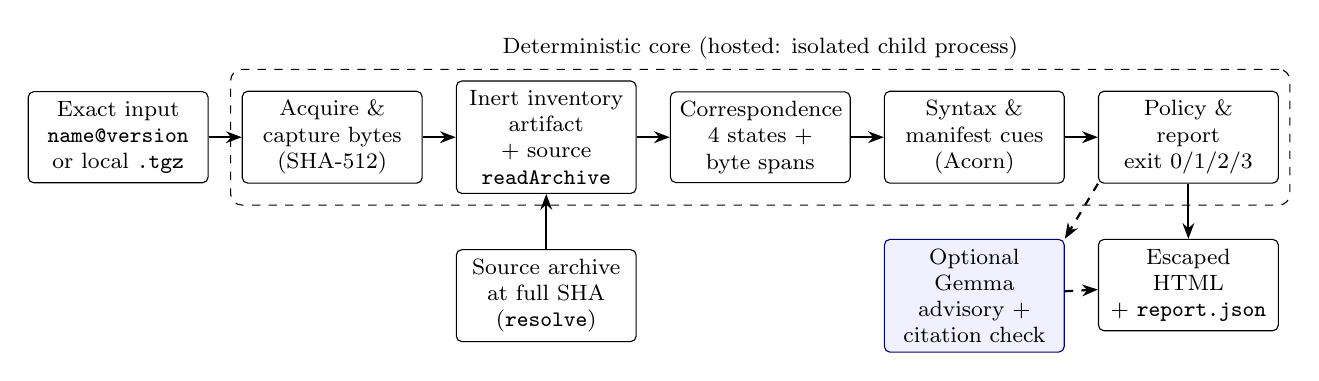
\begin{tikzpicture}[
  node distance=0.45cm and 0.42cm,
  box/.style={draw, rounded corners=2pt, align=center, font=\footnotesize,
              minimum height=0.95cm, text width=2.05cm, fill=white},
  opt/.style={box, fill=blue!6, draw=blue!50!black},
  arr/.style={-{Stealth[length=2mm]}, thick}]
\node[box] (in) {Exact input\\\code{name@version}\\or local \code{.tgz}};
\node[box, right=of in] (acq) {Acquire \&\\capture bytes\\(SHA-512)};
\node[box, right=of acq] (inv) {Inert inventory\\artifact + source\\\code{readArchive}};
\node[box, right=of inv] (cmp) {Correspondence\\4 states +\\byte spans};
\node[box, right=of cmp] (ins) {Syntax \&\\manifest cues\\(Acorn)};
\node[box, right=of ins] (pol) {Policy \&\\report\\exit 0/1/2/3};
\node[box, below=0.7cm of pol] (view) {Escaped HTML\\+ \code{report.json}};
\node[opt, below=0.7cm of ins] (mod) {Optional Gemma\\advisory +\\citation check};
\node[box, below=0.7cm of inv] (src) {Source archive\\at full SHA\\(\code{resolve})};
\draw[arr] (in) -- (acq);
\draw[arr] (acq) -- (inv);
\draw[arr] (inv) -- (cmp);
\draw[arr] (cmp) -- (ins);
\draw[arr] (ins) -- (pol);
\draw[arr] (pol) -- (view);
\draw[arr] (src) -- (inv);
\draw[arr, dashed] (pol.south west) -- (mod.north east);
\draw[arr, dashed] (mod) -- (view);
\node[draw, dashed, rounded corners, inner sep=4pt, fit=(acq)(inv)(cmp)(ins)(pol),
      label={[font=\footnotesize]above:Deterministic core (hosted: isolated child process)}] {};
\end{tikzpicture}
\caption{End-to-end pipeline. The deterministic core fixes the exit code before
the optional model stage (dashed) runs; the model can annotate but never alter
it. Source: \code{docs/architecture.md}.}
\label{fig:pipeline}
\end{figure*}

\subsection{Process Boundaries}
The CLI runs the pipeline in-process. The hosted service separates concerns
across processes: the main process owns HTTP, the queue, the store and the model
client; a trusted Node child runs the deterministic stage with a 512\,MiB V8
old-space limit, a minimal environment and a 120\,s deadline. Provider
credentials stay in the main process and are never inherited by the child. Job
directories have random names and kernel-held ownership leases, so a restart
preserves live jobs and only removes directories it can prove are abandoned.

\subsection{Hosted Job Lifecycle}
A visitor submits \code{name@version} via \code{POST /check}; the server
returns \code{303} to a private \code{/r/<32-hex-id>} location. Jobs move
through \emph{queued} $\to$ \emph{running} $\to$ \{\emph{done},
\emph{incomplete}, \emph{failed}\} and then become unavailable after TTL,
eviction or restart. The queue holds one active and one waiting job; admission
is limited to six new checks per ten minutes; GET requests never start or retry
work.

\section{Methodology}\label{sec:method}

\subsection{Problem Formulation}
Let $A=\{a_1,\dots,a_n\}$ be the regular-file entries of the artifact after
mapping (one validated leading path component stripped), and $S$ the regular
entries of the selected source package directory. Each entry $e$ has a
normalised path $p(e)$, size $|e|$ and digest $h(e)=\mathrm{SHA256}(e)$. Let
$\kappa(S)\in\{0,1\}$ indicate that the source inventory is \emph{complete} and
\emph{unambiguous}, and let $L(p)$ indicate that a source link exists at $p$ or
any ancestor of $p$.

\subsection{Archive Inventory}
\code{readArchive} streams gzip-compressed tar bytes and records, for each
entry, its original and effective path, type, size, SHA-256 and inspection
status. It rejects unsafe paths, unsupported types, traversal, NULs and
canonical collisions, including case-folded and Unicode-normalised collisions:
\begin{equation}
\exists\, e\neq e' : \mathrm{NFC}(\mathrm{fold}(p(e))) = \mathrm{NFC}(\mathrm{fold}(p(e'))) \Rightarrow \text{reject}.
\end{equation}
Content is retained up to 10\,MiB per file within a shared 128\,MiB budget; larger
files are stream-hashed so that no misleading prefix is ever compared.

\subsection{Correspondence Classification}
For each $a\in A$ with counterpart $s\in S$ at the same path, the state is
\begin{equation}
\sigma(a)=\begin{cases}
\textsf{byte-identical} & s \text{ exists},\ |s|=|a|,\ h(s)=h(a)\\
\textsf{changed} & s \text{ exists and usable},\ h(s)\neq h(a)\\
\textsf{artifact-only} & s \text{ absent},\ \kappa(S)=1,\ \neg L(p(a))\\
\textsf{not-compared} & \text{otherwise.}
\end{cases}
\label{eq:states}
\end{equation}
The rule in \eqref{eq:states} is deliberately conservative: absence is asserted
only when the inventory is complete and no link could hide the file, so an
incomplete source can never manufacture an \textsf{artifact-only} finding.
Every artifact file appears exactly once, so
\begin{equation}
\textstyle\sum_{\sigma} N_\sigma = |A|,
\end{equation}
which the report validator checks.

\subsection{Difference Localisation and Evidence}
For a \textsf{changed} file with both sides retained, the first and last
differing byte offsets $i$ and $j$ define a half-open span $[i,j)$ on each side.
An evidence record is the tuple
\begin{equation}
\varepsilon = (\mathit{id},\ \mathrm{SHA256}(\text{blob}),\ \text{side},\ p_{\text{orig}},\ p,\ [i,j)),
\end{equation}
so any claim in the report can be re-checked against the original bytes. When
limits prevent retention, localisation degrades to a whole-file difference
rather than to a guess.

\subsection{Deterministic Policy}
The policy maps a validated report to an exit code
\begin{equation}
c=\begin{cases}
2 & \text{input failure or incomplete analysis}\\
3 & \text{complete, and } F\neq\emptyset\\
0 & \text{complete, and } F=\emptyset
\end{cases}
\end{equation}
with code $1$ reserved for unexpected internal errors. $F$ is the set of
default findings: \code{integrity-mismatch}, \code{identity-claim-conflict},
\code{lifecycle-source-absent} (an install hook in the tarball with no source
counterpart) and \code{lifecycle-implicit-gyp}. Incomplete analysis takes
precedence, and $c$ does not depend on the model. Algorithm~\ref{alg:check}
summarises one check.

\begin{algorithm}[t]
\caption{One UNMASK check}
\label{alg:check}
\begin{algorithmic}[1]
\Require exact spec or tarball $T$; optional source $Z$ at SHA $c$; limits $\Lambda$
\State $b_T \gets$ capture original bytes of $T$; record SHA-512
\State $A \gets \textsc{ReadArchive}(b_T,\ \text{artifact},\ \Lambda)$
\If{$Z$ available} \State $S \gets \textsc{SelectPackage}(\textsc{ReadArchive}(Z,\ \text{source},\ \Lambda))$
\Else \State $S \gets \emptyset$; $\kappa \gets 0$ \EndIf
\For{each regular $a \in A$} \State assign $\sigma(a)$ by \eqref{eq:states}; localise if \textsf{changed} \EndFor
\State $K \gets$ bounded syntax and manifest cues on $A$, $S$
\State $R \gets \textsc{CreateReport}(A, S, \sigma, K)$; $\textsc{Validate}(R)$
\State $c \gets \textsc{Policy}(R)$ \Comment{fixed from here on}
\If{model enabled \textbf{and} consent \textbf{and} eligible evidence}
  \State $H \gets \textsc{Gemma}(\text{bounded evidence})$
  \State keep $h\in H$ only if every quotation matches its evidence span
\EndIf
\State \Return $R$, $H$, $c$
\end{algorithmic}
\end{algorithm}

\subsection{Advisory Model Layer}
The adapter targets \code{gemma-4-26b-a4b-it} on a fixed Google endpoint with
temperature zero, one candidate, at most 4{,}000 input and 1{,}000 output
tokens, and at most two 45\,s attempts. It is disabled unless
\code{UNMASK\_MODEL=on} and verified positive quota limits are configured; the
CLI additionally requires \code{--allow-model}. A hypothesis $h$ is accepted
only if each quotation $q$ it cites satisfies
\begin{equation}
q = \text{bytes}(\varepsilon)[k : k+|q|] \ \text{for some } k,
\end{equation}
for the evidence record $\varepsilon$ it names. This establishes \emph{where}
the model looked, not whether its reasoning is correct; the report says so.

\section{Engineering and Evaluation Design}\label{sec:eng}

\subsection{Resource Budgets}
Table~\ref{tab:limits} lists the source-level defaults. They are budgets, not
measured capacity, and the effective values are recorded in every report so
that two runs can be compared only under the same limits.

\begin{table}[t]
\caption{Default resource budgets (source-level)}
\label{tab:limits}
\centering
\footnotesize
\begin{tabular}{@{}p{2.9cm}p{4.7cm}@{}}
\toprule
\textbf{Area} & \textbf{Default}\\
\midrule
Compressed archive & 50\,MiB each\\
Expanded archive & 250\,MiB; ratio $\le 100$\\
Inventory & 20{,}000 entries; 4{,}096 path bytes\\
Retained content & 10\,MiB/file; 128\,MiB shared\\
Parse / fetch deadline & 30\,s each; redirects refused\\
JavaScript inspection & 2\,MiB/file; 200{,}000 tokens\\
Hosted worker & 512\,MiB V8 heap; 120\,s\\
Queue & 1 active + 1 waiting; 300\,s TTL\\
Admission & 6 checks / 10\,min\\
Report store & 200 entries; 64\,MiB; 24\,h TTL\\
Model & 2$\times$45\,s; 4{,}000 in / 1{,}000 out tokens\\
\bottomrule
\end{tabular}
\vspace{1pt}

\textit{Source:} \code{docs/stack.md}.
\end{table}

\subsection{Continuous Integration}
Every push and pull request runs one job, \emph{Repository checks}, with
\code{contents: read} permission and commit-pinned actions. It (1) installs
the lockfile with \code{npm ci --ignore-scripts}; (2) checks that the running
Node version, \code{.nvmrc}, package engines and lock engines agree and that
direct dependencies are exact versions; (3) syntax-checks every tooling script;
(4) checks Prettier formatting; (5) runs the test suite; (6) reports release
readiness; and (7) inspects the npm archive allowlist. Product build and image
smoke steps run only when readiness is true.

\subsection{Release Integrity}
The release design builds \emph{one} npm tarball, tests the installed tarball,
and builds the container image from those exact bytes. A release manifest binds
version, Git tag, full source SHA, tarball name, size and SHA-256, and the GHCR
image digest. Versions must be strictly greater than every existing stable
version, compared numerically with \code{BigInt} segments; reruns of a used
version are refused, and no step deletes or overwrites a published artifact.
Publishing remains disabled (\code{release.config.json}) until real CLI, server
and website artifacts exist.

\subsection{Testing}
Tests use the built-in \code{node:test} runner~\cite{nodetest}.
Table~\ref{tab:tests} counts test declarations on the merged main branch; several
are parameterised and expand into more cases at run time.

\begin{table}[t]
\caption{Test declarations on main (static count)}
\label{tab:tests}
\centering
\footnotesize
\begin{tabular}{@{}p{3.4cm}cp{3.0cm}@{}}
\toprule
\textbf{File} & \textbf{Decl.} & \textbf{Covers}\\
\midrule
\code{product/shell} & 7 & Escaping, CSP hashes, a11y\\
\code{tooling/build} & 10 & Freshness, stale bytes\\
\code{tooling/release-policy} & 10 & Version order, collisions\\
\code{tooling/readiness} & 5 & Gate prerequisites\\
\code{tooling/candidate} & 3 & Image/archive identity\\
\code{tooling/toolchain} & 3 & Pinned versions\\
\code{tooling/package} & 1 & Archive allowlist\\
\code{tooling/entrypoints} & 2 & Declared entrypoints\\
\code{tooling/docker-context} & 2 & Exact build context\\
\midrule
\textbf{Total} & \textbf{43} & \\
\bottomrule
\end{tabular}
\vspace{1pt}

\textit{Source:} \code{tests/}, counted with \code{grep} on top-level \code{test(} calls.
\end{table}

\subsection{Planned Evaluation Protocol}
Because the analyzer core is not yet on main, no accuracy results are reported
here. The evaluation that will gate Phase~2 is defined in advance:
\begin{itemize}
\item \textbf{Injection benchmark.} Take $N$ popular npm releases with a
resolvable \code{gitHead}; for each, create a modified tarball with one of
$k$ controlled edits (added file, changed byte, added \code{postinstall}). The
detection rate is $\mathrm{TPR}=\mathrm{TP}/(\mathrm{TP}+\mathrm{FN})$ over
modified tarballs, and the clean-release false-finding rate is
$\mathrm{FP}/N$.
\item \textbf{Coverage.} Report the fraction of artifact bytes in each state,
$\sum_{a:\sigma(a)=s}|a| \,/\, \sum_{a}|a|$, since a high
\textsf{not-compared} share means the tool could not judge.
\item \textbf{Cost.} Median and 95th-percentile wall time and peak RSS per check.
\item \textbf{Model usefulness.} Citation-validity rate and a blinded human
rating of whether each accepted hypothesis helps a reviewer.
\end{itemize}

\section{Current Status}\label{sec:status}

Table~\ref{tab:status} reports what exists on the merged main branch at
revision \code{80721ed} and what is pending. The distinction matters: design
documents describe interfaces, not running code.

\begin{table}[t]
\caption{Component status at main revision \code{80721ed}}
\label{tab:status}
\centering
\footnotesize
\begin{tabular}{@{}p{2.6cm}p{1.5cm}p{3.5cm}@{}}
\toprule
\textbf{Component} & \textbf{State} & \textbf{Evidence}\\
\midrule
CI workflow & Merged & \code{.github/workflows/ci.yml}\\
Release tooling & Merged, gated & \code{scripts/release*.mjs}; publishing off\\
Website shell & Merged & \code{src/viewer/shell.mjs}, 7 tests\\
Package identity & Merged & \code{@xagents\_in/unmask}, private 0.0.0\\
Design \& contracts & Merged & \code{docs/*.md}\\
Analyzer core & Pending & Specified; not on main\\
HTTP server, CLI & Pending & Specified; not on main\\
Hosted model & Blocked & Generation returned HTTP 403\\
Deployment & Not started & No image or service\\
\bottomrule
\end{tabular}
\end{table}

\textbf{Model diagnostic.} A minimal metadata lookup and token-counting request
to \code{gemma-4-26b-a4b-it} succeeded. Generation returned HTTP~403
\code{PERMISSION\_DENIED} because the configured project's free tier is
unavailable. No generated output was obtained, no package evidence was sent, and
no billing change was made. The model acceptance gate is therefore unmet.

\textbf{Repository activity.} The main branch has 22 commits from four
contributors, merged through six pull requests that follow the repository's
four-section PR template (what the PR does, models used, testing, risks).

\section{Discussion}\label{sec:disc}

\subsection{Answers to the Design Questions}
\textbf{DQ1: Inert comparison.} The specification shows that a useful
comparison needs no execution: byte digests, conservative absence rules and
byte spans are enough to separate identical, changed and extra files, and
install hooks can be read from manifests. Whether this is useful \emph{in
practice} depends on how often packages ship generated code with no source
counterpart; LastPyMile~\cite{vu2021} suggests often, which is why
\textsf{not-compared} and coverage are reported rather than hidden.

\textbf{DQ2: Separated facts.} Table~\ref{tab:facts} answers this directly.
The key rule is asymmetric: weaker facts may \emph{prioritise} review but never
\emph{clear} a stronger finding.

\textbf{DQ3: Model role.} The model can add value only as an explainer whose
quotations are checked and whose output cannot change the exit code. Even this
narrow role is not yet validated, because generation is blocked.

\subsection{Why Not the Alternatives}
\emph{Rebuild and compare}~\cite{lamb2021} gives stronger guarantees but
executes untrusted build scripts and needs a faithful toolchain for every
package; it is a natural extension once the inert core is proven.
\emph{Trust provenance alone}~\cite{npmprov} covers only packages that publish
it, and the current acquisition path does not verify signatures, so treating it
as proof would overstate assurance. \emph{AST or semantic diff} could explain
minified changes but cannot establish equivalence in general and would enlarge
the attack surface of the parser. \emph{LLM as classifier} would be fast to
demonstrate but would make the verdict depend on an unvalidated, non-deterministic
component, contradicting DQ2.

\subsection{Threats to Validity}
\textbf{Construct validity.} Byte identity is a strict notion of
correspondence; a benign rebuild that changes a timestamp is reported as
\textsf{changed}. This is intended, but it will raise the share of findings a
reviewer must inspect. \textbf{Internal validity.} This report relies on design
documents for the core; the code that implements them has been reviewed locally
by the team but is not yet public. \textbf{External validity.} Scope is npm
only; PyPI and other ecosystems have different packaging conventions.

\section{Limitations and Future Work}\label{sec:future}

Each item states a measurable test of completion.

\textbf{Merge the analyzer core.} Land \code{core/}, \code{cli/} and
\code{server/} with product tests. \emph{Done when} \code{npm run test:product}
runs in CI and \code{release:readiness} reports no product blockers.

\textbf{Unblock the model.} Obtain a quota-verified Gemma configuration.
\emph{Done when} one end-to-end check produces a validated advisory section and
a human reviewer rates it.

\textbf{Run the injection benchmark.} \emph{Done when} TPR, false-finding rate,
coverage and latency are reported for at least 100 releases.

\textbf{Verify provenance.} Implement Sigstore verification for npm
provenance~\cite{sigstore,npmprov}. \emph{Done when}
\code{provenance-verification-failed} is emitted by a real verifier.

\textbf{Deploy.} Build the image from the released tarball and deploy to the
selected DigitalOcean App Platform service. \emph{Done when} \code{/version}
returns the manifest's commit and tarball hash.

\textbf{Extend scope.} Add PyPI wheels and source distributions. \emph{Done when}
the injection benchmark runs on PyPI releases.

\section{Conclusion}

UNMASK addresses a gap that registries leave open: the published package and
the reviewed source are separate artifacts, and nothing checks that they agree.
The project's main contribution so far is a precise, bounded and non-executing
design that keeps every fact at its true strength, ties every claim to bytes,
and keeps the verdict independent of the language model. The engineering
foundation that will carry it --- pinned toolchain, read-only CI, gated and
digest-bound releases, and an accessible escaped website shell --- is merged and
tested. The analyzer core, model acceptance and the evaluation benchmark are the
work of the next phase, and their completion criteria are defined above.

\appendices

\section{Repository Structure and Reproduction}
The repository has six top-level parts. \code{docs/} holds the architecture,
contracts, stack, release and website documentation. \code{scripts/} holds the
build, package, toolchain, readiness, release-policy and candidate tooling.
\code{src/viewer/} holds the website shell. \code{tests/} holds tooling and
product tests. \code{.github/} holds the CI and release workflows, the
\code{CODEOWNERS} file and the PR template. \code{report/} holds this report's
LaTeX source. Reproduction requires Node.js~24.22.2 and the commands
\code{npm ci --ignore-scripts}, \code{npm run check}, \code{npm test} and
\code{npm run check:package}.

\section{Individual Contributions}

\begin{center}
\footnotesize
\begin{tabular}{@{}p{2.3cm}p{5.4cm}@{}}
\toprule
\textbf{Member} & \textbf{Primary responsibilities}\\
\midrule
\AuthorOneName & \textit{\AuthorOneWork}\\
\AuthorTwoName & \textit{\AuthorTwoWork}\\
\AuthorThreeName & \textit{\AuthorThreeWork}\\
\AuthorFourName & \textit{\AuthorFourWork}\\
\bottomrule
\end{tabular}
\end{center}

\section*{Acknowledgment}
The authors thank the organisers of Hacktoberfest 2026 Hack Day Sonipat and the
faculty of Newton School of Technology, Rishihood University, for guidance, and
the maintainers of Node.js, \code{tar-stream} and Acorn.

\begin{thebibliography}{00}
\bibitem{eventstream} npm, Inc., ``Details about the event-stream incident,'' \emph{The npm Blog}, Nov. 2018.
\bibitem{xz} NIST, ``CVE-2024-3094: Malicious code in xz-utils upstream tarballs,'' National Vulnerability Database, 2024.
\bibitem{sigstore} Z. Newman, J. S. Meyers, and S. Torres-Arias, ``Sigstore: Software signing for everybody,'' in \emph{Proc. ACM SIGSAC Conf. Computer and Communications Security (CCS)}, 2022, pp. 2353--2367.
\bibitem{intoto} S. Torres-Arias, H. Afzali, T. K. Kuppusamy, R. Curtmola, and J. Cappos, ``in-toto: Providing farm-to-table guarantees for bits and bytes,'' in \emph{Proc. 28th USENIX Security Symp.}, 2019, pp. 1393--1410.
\bibitem{slsa} OpenSSF, ``Supply-chain Levels for Software Artifacts (SLSA), specification v1.0,'' 2023. [Online]. Available: \url{https://slsa.dev}
\bibitem{npmprov} GitHub, ``Generating provenance statements,'' \emph{npm Docs}, 2023. [Online]. Available: \url{https://docs.npmjs.com/generating-provenance-statements}
\bibitem{lamb2021} C. Lamb and S. Zacchiroli, ``Reproducible builds: Increasing the integrity of software supply chains,'' \emph{IEEE Software}, vol. 39, no. 2, pp. 62--70, 2022.
\bibitem{zimmermann2019} M. Zimmermann, C.-A. Staicu, C. Tenny, and M. Pradel, ``Small world with high risks: A study of security threats in the npm ecosystem,'' in \emph{Proc. 28th USENIX Security Symp.}, 2019, pp. 995--1010.
\bibitem{ohm2020} M. Ohm, H. Plate, A. Sykosch, and M. Meier, ``Backstabber's knife collection: A review of open source software supply chain attacks,'' in \emph{Proc. DIMVA}, LNCS 12223, 2020, pp. 23--43.
\bibitem{duan2021} R. Duan, O. Alrawi, R. P. Kasturi, R. Elder, B. Saltaformaggio, and W. Lee, ``Towards measuring supply chain attacks on package managers for interpreted languages,'' in \emph{Proc. NDSS}, 2021.
\bibitem{vu2021} D.-L. Vu, F. Massacci, I. Pashchenko, H. Plate, and A. Sabetta, ``LastPyMile: Identifying the discrepancy between sources and packages,'' in \emph{Proc. ESEC/FSE}, 2021, pp. 780--792.
\bibitem{ji2023} Z. Ji \emph{et al.}, ``Survey of hallucination in natural language generation,'' \emph{ACM Computing Surveys}, vol. 55, no. 12, pp. 1--38, 2023.
\bibitem{gao2023} T. Gao, H. Yen, J. Yu, and D. Chen, ``Enabling large language models to generate text with citations,'' in \emph{Proc. EMNLP}, 2023, pp. 6465--6488.
\bibitem{gemma} Gemma Team, Google DeepMind, ``Gemma: Open models based on Gemini research and technology,'' arXiv preprint arXiv:2403.08295, 2024.
\bibitem{nodetest} OpenJS Foundation, ``Node.js test runner (\texttt{node:test}),'' Node.js v24 documentation, 2025.
\bibitem{tarstream} M. Buus, ``tar-stream: A streaming tar parser and generator,'' v3.2.2. [Online]. Available: \url{https://github.com/mafintosh/tar-stream}
\bibitem{acorn} M. Haverbeke \emph{et al.}, ``Acorn: A small, fast JavaScript-based JavaScript parser,'' v8.19.0. [Online]. Available: \url{https://github.com/acornjs/acorn}
\end{thebibliography}

\end{document}
